The goal of \FiPy{} is to provide a highly customizable, open source
code for modeling problems involving coupled sets of PDEs.  \FiPy{}
allows users to select and customize modules from within the
framework.  \FiPy{} has been developed to address model problems in
materials science such as poly-crystals, dendritic growth and
electrochemical deposition.  These applications all contain various
combinations of PDEs with differing forms in conjunction with other
unusual physics (over varying length scales) and unique solution
procedures.  The philosophy of \FiPy{} is to enable customization
while providing a library of efficient modules for common objects and
data types.

\section{Design}

\subsection{Numerical Approach}

The solution algorithms given in the \FiPy{} examples involve combining
sets of PDEs while tracking an interface where the parameters of the
problem change rapidly. The phase field method and the level set
method are specialized techniques to handle the solution of
PDEs in conjunction with a deforming interface. \FiPy{} contains
several examples of both methods.

\FiPy{} uses the well-known Finite Volume Method (FVM) to reduce the
model equations to a form tractable to linear solvers.

\subsection{Object Oriented Structure}

\FiPy{} is programmed in an object-oriented manner.  The benefit of
object oriented programming mainly lies in encapsulation and
inheritance.  Encapsulation refers to the tight integration between
certain pieces of data and methods that act on that data.
Encapsulation allows parts of the code to be separated into clearly
defined independent modules that can be re-applied or extended in new
ways.  Inheritance allows code to be reused, overridden, and new
capabilities to be added without altering the original code. An object
is treated by its users as an abstraction; the details of its
implementation and behavior are internal.

\subsection{Test Based Development}

\FiPy{} has been developed with a large number of test cases.  These
test cases are in two categories.  The lower level tests operate on
the core modules at the individual method level.  The aim is that
every method within the core installation has a test case.  The high
level test cases operate in conjunction with example solutions and
serve to test global solution algorithms and the interaction of
various modules.  

With this two-tiered battery of tests, at any stage in code
development, the test cases can be executed and errors can be
identified.  A comprehensive test base provides reassurance that any
code breakages will be clearly demonstrated with a broken test case.
A test base also aids dissemination of the code by providing simple
examples and knowledge of whether the code is working on a particular
computer environment.

\subsection{Open Source}

In recent years, there has been a movement to release software under
open source and associated unrestrictied licenses, especially within
the scientific community.  These licensing terms allow users to
develop their own applications with complete access to the source code
and then either contribute back to the main source repository or
freely distribute their new adapted version.  

As a product of the National Institute of Standards and Technology,
the \FiPy{} framework is placed in the public domain as a matter of U.
S. Federal law. Furthermore, \FiPy{} is built upon existing open source 
tools. Others are free to use \FiPy{} as they see fit and we welcome
contributions to make \FiPy{} better.

\subsection{High-Level Scripting Language}

Programming languages can be broadly lumped into two categories:
compiled languages and interpreted (or scripting) languages.  Compiled
languages are converted from a human-readable text source file to a
machine-readable binary application file by a sequence of operations
generally referred to as ``compiling'' and ``linking''.  The binary
application can then be run as many times as desired, but changes will
provoke a new cycle of compiling and linking.  Interpreted languages
are converted from human-readable to machine-readable on the fly, each
time the script is executed.  Because the conversion happens every
time\footnote{\ldots neglecting such common optimizations as byte-code
interpreters}, interpreted code is usually slower when running than
compiled code.  On the other hand, code development and debugging
tends to be much easier and fluid when it's not necessary to wait for
compile and link cycles after every change.  Furthermore, because the
conversion happens in real time, it is possible to have interactive
sessions in a scripting language that are not generally possible in
compiled languages.

Another distinction, somewhat orthogonal, but closely related, to that
between compiled and interpreted languages, is between low-level
languages and high-level languages.  Low-level languages describe
actions in simple terms that are closer to the way the computer actually
functions.  High-level languages describe actions in more complex and
abstract terms that are closer to the way the programmer thinks about
the problem at hand.  This increased complexity in the meaning of an
expression renders simpler code, because the details of the
implementation are hidden away in the language internals or in an
external library.  For example, a low-level matrix multiplication
written in C might be rendered as
\begin{quote}
\begin{verbatim}
if (Acols != Brows) 
    error "these matrix shapes cannot be multiplied";

C = (float *) malloc(sizeof(float) * Bcols * Arows);

for (i = 0; i < Bcols; i++) {
    for (j = 0; j < Arows; j++) {
        C[i][j] = 0;
        for (k = 0; k < Acols; k++) {
            C[i][j] += A[i][k] * B[k][j];
        }
    }
}
\end{verbatim}
\end{quote}
Note that the dimensions of the arrays must be supplied externally, as
C provides no intrinsic mechanism for determining the shape of an
array.  An equivalent high-level construction might be as simple as
\begin{quote}
\begin{verbatim}
C = A * B
\end{verbatim}
\end{quote}
All of the error checking, dimension measuring, and space allocation
is handled automatically by low-level code that is intrinsic to the
high-level matrix multiplication operator.  The high-level code
``knows'' that matrices are involved, how to get their shapes, and to
interpret `\verb|*|' as a matrix multiplier instead of an arithmetic
one.  All of this allows the programmer to think about the operation
of interest and not worry about introducing bugs in low-level code
that is not unique to their application.

Although it needn't be true, for a variety of reasons, compiled
languages tend to be low-level and interpreted languages tend to be
high-level.  Because low-level languages operate closer to the
intrinsic ``machine language'' of the computer, they tend to be faster
at running a given task than high-level languages, but programs
written in them take longer to write and debug.  Because running
performance is a paramount concern, most scientific codes are written
in low-level compiled languages like FORTRAN or C.

A rather common scenario in the development of scientific codes is
that the first draft hard-codes all of the problem parameters.  After
a few (hundred) iterations of recompiling and relinking the
application to explore changes to the parameters, code is added to
read an input file containing a list of numbers.  Eventually, the
point is reached where it is impossible to remember which parameter
comes in which order or what physical units are required, so code is
added to, for example, interpret a line beginning with `\verb|#|' as a
comment.  At this point, the scientist has begun developing a
scripting language without even knowing it.  Unfortunately for them,
very few scientists have actually studied computer science or actually
know anything about the design and implementation of script
interpreters.  Even if they have the expertise, the time spent
developing such a language interpreter is time not spent actually
doing research.

In contrast, a number of very powerful scripting languages, such as
Tcl, Java, Python, Ruby, and even the venerable BASIC, have open
source interpreters that can be embedded directly in an application,
giving scientific codes immediate access to a high-level scripting
language designed by someone who actually knew what they were doing.

We have chosen to go a step further and not just embed a full-fledged
scripting language in the \FiPy{} framework, but instead to design the
framework from the ground up in a scripting language.  While runtime
performance is unquestionably important, many scientific codes are run
relatively little, in proportion to the time spent developing them.
If a code can be developed in a day instead of a month, it may not
matter if it takes another day to run instead of an hour.
Furthermore, there are a variety of mechanisms for diagnosing and
optimizing those portions of a code that are actually time-critical,
rather than attempting to optimize all of it by using a language that
is more palatable to the computer than to the programmer.  Thus
\FiPy{}, rather than taking the approach of writing the fast numerical
code first and then dealing with the issue of user interaction,
initially implements most modules in high-level scripting language and
only translates to low-level compiled code those portions that prove
inefficient. A discussion of efficiency issues can be found in
Chapter~\ref{chap:Efficiency}.

\subsection{\Python{} Programming Language}

Acknowledging that several scripting languages offer a number, if not
all, of the features described above, we have selected \Python{} for
the implementation of \FiPy{}.  Python is:
\begin{itemize}
    
    \item an interpreted language that combines remarkable power with very clear
    syntax,
    
    \item freely usable and distributable, even for commercial use,
    
    \item fully object oriented,
    
    \item distributed with powerful automated testing tools (\doctest{},
    \unittest{}),

    \item actively used and extended by other scientists and
    mathemeticians (\SciPy{}, \Numeric{}, \ScientificPython{}, \PySparse{}).
    
    \item easily integrated with low-level languages such as C
    (\weave{}, \blitz{}, \PyRex{}).
    
\end{itemize}

\section{Implementation}

The \Python{} classes that make up \FiPy{} are described in detail in
the \href{file:reference.pdf}{\textit{\FiPy{} Programmer's
Reference}}, but we give a brief overview here.  \FiPy{} is based
around three fundamental \Python{} classes: \Class{Mesh},
\Class{Variable}, and \Class{Term}.  Using the terminology of
Chapter~\ref{chap:Numerics}:
\begin{description}
    \item[A \Class{Mesh} object] represents the domain of interest.
    \FiPy{} contains many different specific mesh classes to describe
    different geometries.

    \item[A \Class{Variable} object] represents a quantity or field
    that can change during the problem evolution.  A particular type
    of \Class{Variable}, called a \Class{CellVariable}, represents \(
    \phi \) at the centers of the \Class{Cell}s of the \Class{Mesh}.
    A \Class{CellVariable} describes the values of the field \( \phi
    \), but it is not concerned with their geometry; that role is
    taken by the \Class{Mesh}.

    An important property of \Class{Variable} objects is that they can
    describe dependency relationships, such that:    
\begin{quote}
\begin{verbatim}
>>> a = Variable(value = 3)
>>> b = a * 4
\end{verbatim}
\end{quote}
    does not assign the value \verb|12| to \verb|b|, but rather it
    assigns a multiplication operator object to \verb|b|, which
    depends on the \Class{Variable} object \verb|a|:
\begin{quote}
\begin{verbatim}
>>> b
(Variable(value = 3) * 4)
>>> a.setValue(5)
>>> b
(Variable(value = 5) * 4)
\end{verbatim}
\end{quote}
    The numerical value of the \Class{Variable} is not calculated
    until it is needed (a process known as ``lazy evaluation''):
\begin{quote}
\begin{verbatim}
>>> print b
20
\end{verbatim}
\end{quote}

    \item[A \Class{Term} object] represents any of the terms in
    Equation~\eqref{eqn:num:gen} or any linear combination of such
    terms.  Early in the development of \FiPy{}, a distinction was
    made between \Class{Equation} objects, which represented all of
    Equation~\eqref{eqn:num:gen}, and \Class{Term} objects, which
    represented the individual terms in that equation.  The
    \Class{Equation} object has since been eliminated as redundant.
    \Class{Term} objects can be single entities such as an
    \Class{ImplicitDiffusionTerm} or a linear combination of other
    \Class{Term} objects that build up to form an expression such as
    Equation~\eqref{eqn:num:gen}.
    
%     The different \Class{Term} objects used to represent PDEs in
%     \FiPy{} are introduced in the different physical problems of
%     Part~\ref{part:Examples}, but we present a general discussion of
%     their form here.  As explained in Chapter~\ref{chap:Numerics}, the
%     canonical governing equation that can be solved by \FiPy{} for the
%     dependent \Class{CellVariable} $\phi$ is
%     \begin{equation}                        
%          \underbrace{
%            \frac{\partial (\rho \phi)}{\partial t}
%          }_{\text{transient}}
%          =
%          \underbrace{
%            \vphantom{\frac{\partial (\rho \phi)}{\partial t}}
%            \nabla \cdot \left( \vec{u} \phi \right)
%          }_{\text{convection}}
%          +
%          \underbrace{
%            \vphantom{\frac{\partial (\rho \phi)}{\partial t}}
%            \nabla \cdot \left( \Gamma_1 \nabla \phi \right) 
%          }_{\text{diffusion}}
%          +
%          \underbrace{
%            \vphantom{\frac{\partial (\rho \phi)}{\partial t}}
%            \left[ \nabla \cdot \left( \Gamma_i \nabla \right) \right]^n \phi
%          }_{\text{$n$\textsuperscript{th} order}}
%          +
%          \underbrace{
%            \vphantom{\frac{\partial (\rho \phi)}{\partial t}}
%            S_{\phi}
%          }_{\text{source}}
%          \tag{\ref{eqn:num:gen}}
%     \end{equation}
%     A physical problem can involve many different coupled governing
%     equations, one for each variable.
%     
%     Let us examine this expression term-by-term:
%     \begin{description}
%         \item[Transient Term] 
%           $$\frac{\partial (\rho \phi)}{\partial t}$$ 
%           is obtained in \FiPy{} by
%           \begin{quote}
% \begin{verbatim}
% >>> TransientTerm(coeff = rho)
% \end{verbatim}
%           \end{quote}
%         
%           \begin{reSTadmonition}[Note]
%               We have specified neither the variable $\phi$ nor the time
%               step.  Both are handled when we actually solve the equation.
%           \end{reSTadmonition}
%           
%          \item[Convection Term]
%            $$\nabla \cdot \left( \vec{u} \phi \right)$$ 
%            is obtained by
%            \begin{quote}
% \begin{verbatim}
% >>> <Specific>ConvectionTerm(coeff = u, 
% ...                          diffusionTerm = diffTerm)
% \end{verbatim}
%            \end{quote}
%            where \verb|<Specific>| can be any of \verb|CentralDiff|,
%            \verb|Exponential|, \verb|Hybrid|, \verb|PowerLaw|,
%            \verb|Upwind|, \verb|ExplicitUpwind|, or \verb|VanLeer|.
%            The differences between these convection schemes are described
%            in Section~\ref{sec:NumericalSchemes}. The velocity coefficient 
%            \verb|u| must be a \Class{FaceVectorVariable}, or a 
%            constant vector in the form of a Python list or tuple, 
%            \emph{e.g.} \verb|(1,2)| for a vector in 2D.
%            
%            \begin{reSTadmonition}[Note]
%                As discussed in Section~\ref{sec:NumericalSchemes}, the
%                convection schemes need to calculate a P\'eclet number,
%                and therefore need to know about any diffusion term
%                used in the problem.  It is hoped that this dependency
%                can be automated in the future.
%            \end{reSTadmonition}
%            
%            \begin{reSTadmonition}[Warning]
%                \Class{VanLeerConvectionTerm} not mentioned and no discussion of
%                explicit forms.
%            \end{reSTadmonition}
%           
%         \item[Diffusion Term]
%           $$\nabla \cdot \left( \Gamma_1 \nabla \phi \right)$$
%           is obtained by either
%           \begin{quote}
% \begin{verbatim}
% >>> ImplicitDiffusionTerm(coeff = Gamma1)
% \end{verbatim}
%           \end{quote}
%           or 
%           \begin{quote}
% \begin{verbatim}
% >>> ExplicitDiffusionTerm(coeff = Gamma1)
% \end{verbatim}
%           \end{quote}
%           \Class{ExplicitDiffusionTerm} is provided only for illustrative purposes.
%           \Class{ImplicitDiffusionTerm} is almost always preferred. It is
%           theoretically possible to create an explicit diffusion term with
%           \begin{quote}
% \begin{verbatim}
% >>> (Gamma1 * phi.getFaceGrad()).getDivergence()
% \end{verbatim}
%           \end{quote}
%           Unfortunately, in this form, any boundary conditions on $\phi$
%           will not be accounted for.
%           
%         \item[$n$\textsuperscript{th}-Order Diffusion Term]
%           $$\nabla \cdot \left\{ \Gamma_1 \nabla \left[ \nabla\cdot\left( 
%           \Gamma_2 \nabla \phi\right) \right] \right\}$$
%           is obtained by
%           \begin{quote}
% \begin{verbatim}
% >>> NthOrderDiffusionTerm(coeff = (Gamma1, Gamma2))
% \end{verbatim}
%           \end{quote}
%           The number of elements supplied for \verb|coeff| determines the
%           order of the term. As such,
%           \begin{quote}
% \begin{verbatim}
% >>> NthOrderDiffusionTerm(coeff = Gamma1)
% \end{verbatim}
%           \end{quote}
%           is completely equivalent to
%           \begin{quote}
% \begin{verbatim}
% >>> ImplicitDiffusionTerm(coeff = Gamma1)
% \end{verbatim}
%           \end{quote}
%           
%         \item[Source Term]
%           Any terms that cannot be written in one of the previous forms is
%           considered a source $S_{\phi}$. 
%           An explicit source is written in Python essentially as it appears in
%           mathematical form, \emph{e.g.}, $3\kappa^2 + b \sin \theta$
%           would be written
%           \begin{quote}
% \begin{verbatim}
% >>> 3 * kappa**2 + b * sin(theta)
% \end{verbatim}
%           \end{quote}
%           If, however, the source depends on the variable that is being solved for,
%           it can be advantageous to linearize the source and cast part of it as an
%           implicit source term, \emph{e.g.}, $3\kappa^2 + \phi \sin \theta$
%           might be written as
%           \begin{quote}
% \begin{verbatim}
% >>> 3 * kappa**2 + ImplicitSourceTerm(coeff = sin(theta))
% \end{verbatim}
%           \end{quote}
%           
%           \begin{reSTadmonition}[Warning]
%               There are subtleties in properly linearizing a source term
%               which are examined in
%               Example~\ref{examples:phase:simple:input}.
%           \end{reSTadmonition}
%           
%           It is important to realize that, even though an expression may
%           superficially resemble one of those shown above, if the
%           dependent variable \emph{for that PDE} does not appear in the
%           appropriate place, then that term should be treated as a source.
%           \begin{description}
%               \item[Diffusive Source]
%                   For example, if the governing equation for $\phi$ is
%                   \[
%                       \frac{\partial \phi}{\partial t} 
%                       = \nabla\cdot\left( D_1 \nabla \phi\right)
%                       + \nabla\cdot\left( D_2 \nabla \xi\right)
%                   \]
%                   then the first term is a \Class{TransientTerm} and the second term 
%                   is an \Class{ImplicitDiffusionTerm}, but the third term is 
%                   simply an explicit source, which is written in Python as
%                   \begin{quote}
% \begin{verbatim}
% >>> (D2 * xi.getFaceGrad()).getDivergence()
% \end{verbatim}
%                   \end{quote}
%                   
%                   \begin{reSTadmonition}[Note]
%                       We use \verb|getFaceGrad()|, rather than
%                       \verb|getGrad()|, in order to obtain a
%                       second-order diffusion term in $\xi$, consistent
%                       with the matrix that is formed by
%                       \Class{ImplicitDiffusionTerm} for $\phi$.
%                   \end{reSTadmonition}
% 
%               \item[Convective Source]
%                   The convection of an independent field $\xi$ in
%                   \[
%                       \frac{\partial \phi}{\partial t} 
%                       = \nabla\cdot
%                       \left(
%                           \vec{u} \xi
%                       \right)
%                   \]
%                   can be renderd as
%                   \begin{quote}
% \begin{verbatim}
% >>> (uFaceVector * xi.getArithmeticFaceValue()).getDivergence()
% \end{verbatim}
%                   \end{quote}
%                   or it can be factored as
%                   \begin{quote}
% \begin{verbatim}
% >>> uFaceVector.getDivergence() * xi + uFaceVector.dot(xi.getFaceGrad())
% \end{verbatim}
%                   \end{quote}
% 
%               \item[Transient Source]
%                   The time-rate-of change of an independent variable $\xi$, such 
%                   as in
%                   \[
%                       \frac{\partial (\rho_1 \phi)}{\partial t}
%                       = \frac{\partial (\rho_2 \xi)}{\partial t}
%                   \]
%                   does not have an abstract form in \FiPy{} and should be
%                   discretized directly, in the manner of
%                   Equation~\eqref{eqn:num:tra}, as
%                   \begin{quote}
% \begin{verbatim}
% >>> TransientTerm(coeff = rho1) == rho2 * (xi - xi.getOld()) / timeStep
% \end{verbatim}
%                   \end{quote}
%                   This technique is used in Example~\ref{examples:phase:anisotropy:input}.
%           \end{description}
%     \end{description}
% 
%     Since an equation can be composed from \Class{Term} objects in a variety of 

\end{description}

Beyond these three fundamental classes of \Class{Mesh}, 
\Class{Variable}, and \Class{Term}, \FiPy{} is composed of a
number of related classes. The relationships between these classes are shown in
Figure~\ref{fig:objects}. 
\begin{figure}[tbp]
    \centering
    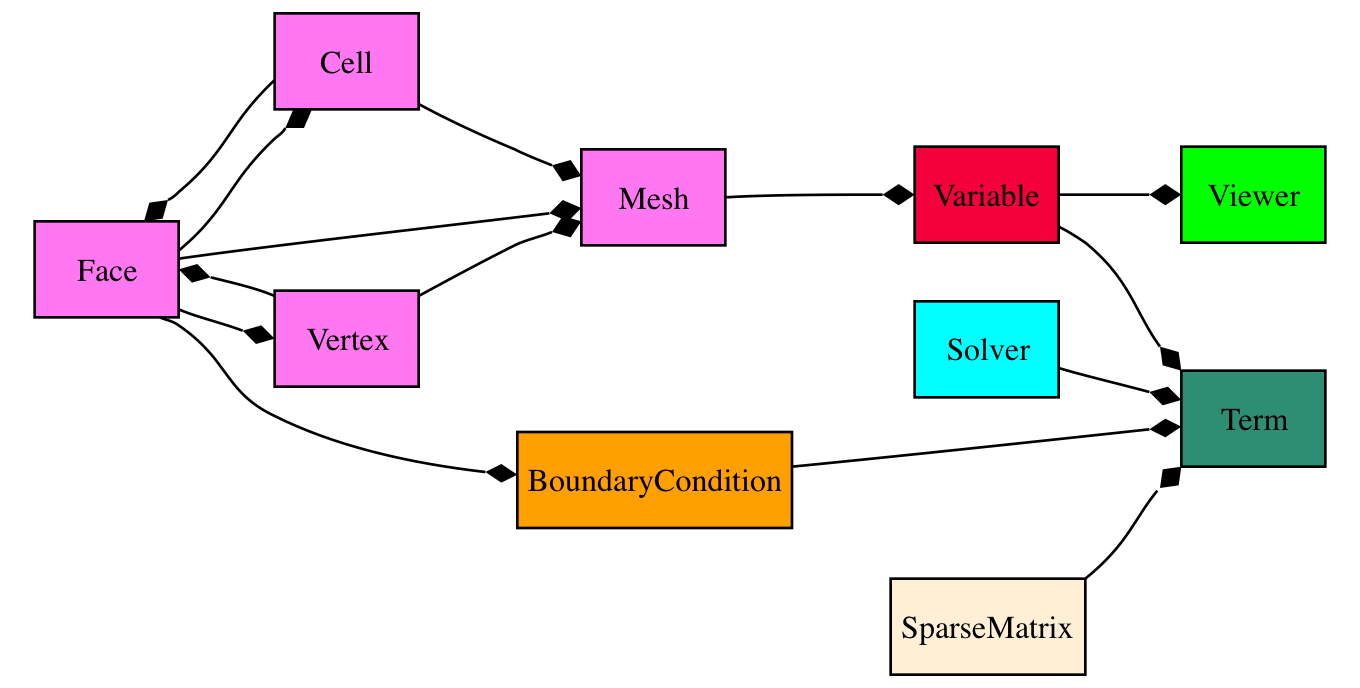
\includegraphics[width=0.9\textwidth]{objects}
    \caption{Primary object relationships in \FiPy{}.}
    \label{fig:objects}
\end{figure}
A \Class{Mesh} object is composed of \Class{Cell} objects.  Each
\Class{Cell} is defined by its bounding \Class{Face} objects and each
\Class{Face} is defined by its bounding \Class{Vertex} objects.  A
\Class{Term} object encapsulates the contributions to the
\Class{SparseMatrix} that defines the solution of an equation.
\Class{BoundaryCondition} objects are used to describe the conditions
on the boundaries of the \Class{Mesh}, and each \Class{Term}
interprets the \Class{BoundaryCondition} objects as necessary to
modify the \Class{SparseMatrix}.  An equation constructed from
\Class{Term} objects can apply a unique \Class{Solver} to invert its
\Class{SparseMatrix} in the most expedient and stable fashion.  At any
point during the solution, a \Class{Viewer} can be invoked to display
the values of the solved \Class{Variable} objects.

At this point, it will be useful to examine some of the example
problems in Part~\ref{part:Examples}.  More classes are introduced in
the examples, along with illustrations of their instantiation and use.


